% !TEX root =  ../Dissertation.tex

\chapter{Design}

The design section describes the systems needed to extract the dependency
graphs and analyse them. Agda Tree analyses two dependencies graphs, one for
modules and another for definitions. The module dependency graph can be
generated with Agda but for the definition dependency graph is created
manually.

Agda Comp is a simpler tool, as the complexity comes from testing the different
compilation strategies. It creates the module dependency graph, apply the
given strategy using the parameters provided by the user, and compile with the
order. 

\pagebreak

\section{Agda Tree}

Agda Tree is a CLI that lets the user interact with the
module and definition graphs. The first command designed is how the both
dependency graphs are created. \cref{fig:Agda Create Tree Diagram} illustrates
how the user will interact with the CLI to create the graphs. The user provides
the Agda file that they want to analyse, normally this would be the entire
everything index file. The everything index file is the file that imports all
the modules in a project. This is standard in Agda, as this is the only way to
type-check the whole project. Depending on the Agda project, this file will be
generated automatically or by the project maintainers.
\begin{figure}[H]
    \centering
    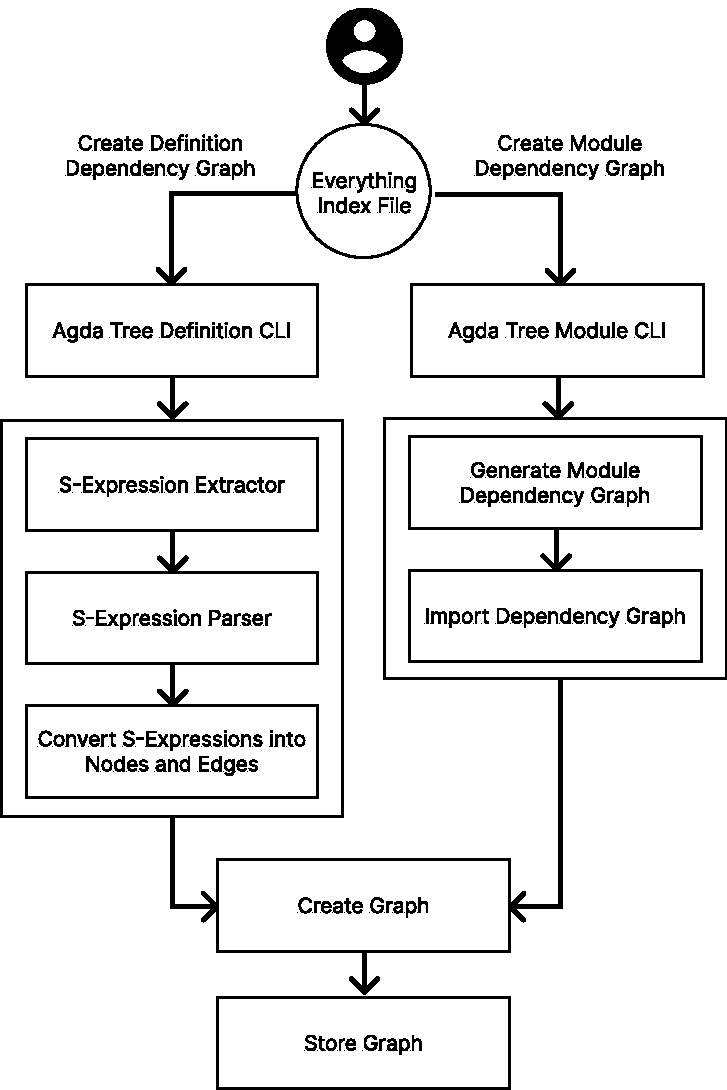
\includegraphics[scale=0.8]{Agda Create Tree.pdf}
    \caption{Agda Create Tree Diagram}
    \label{fig:Agda Create Tree Diagram}
\end{figure} 

\pagebreak

\cref{fig:Agda Tree Class Diagram} is a Class Diagram, showing the classes and
methods to operate the command-line. The CLI parses the input by the user and
delegates the query to the respective dependency graph. Each dependency graph
allows for a different set of queries. These queries can be found in
\cref{tbl:Definition Graph Queries} for the definition graph and in
\cref{tbl:Module Graph Queries} for the module graph.

The definition graph creation depends on the s-expression extractor and parser.
They read the Agda projects and convert the data found into the dependency
graph.

\begin{figure}[H]
    \centering
    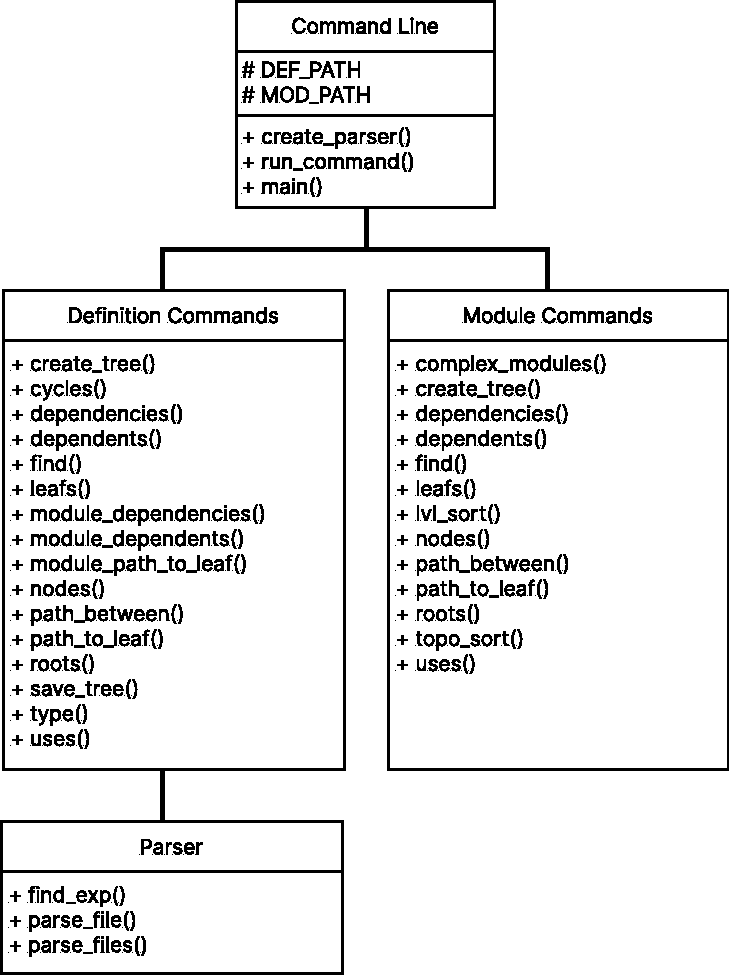
\includegraphics[scale=0.8]{Agda Tree Class Diagram.pdf}
    \caption{Agda Tree Class Diagram}
    \label{fig:Agda Tree Class Diagram}
\end{figure} 
    
\pagebreak

\cref{fig:Agda Tree Query Diagram} shows how is split CLI into two, depending
on what dependency graph is being queried. When the user makes a query, they
will select the dependency graph and the respective queries will perform that
query. The output will be displayed in stdout, which can be used with other
operations like piping and xargs.

\begin{figure}[H]
    \centering
    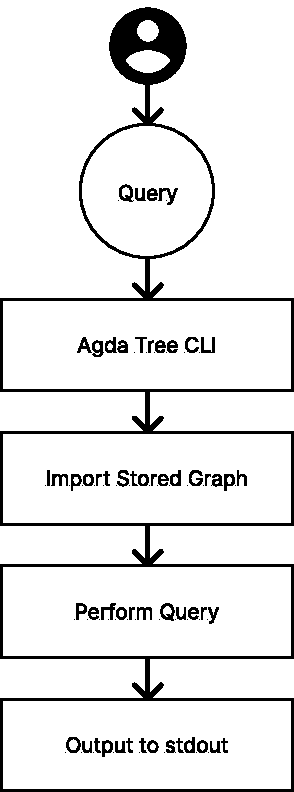
\includegraphics[scale=0.8]{Agda Make Query.pdf}
    \caption{Agda Tree Query Diagram}
    \label{fig:Agda Tree Query Diagram}
\end{figure} 

\pagebreak 


\section{Agda Comp}

\cref{fig:Agda Comp Diagram} demonstrates how the user will interact with
the Agda Comp tool. The user provides the module that to be compiled, next to some
parameters defining the amount of cores used in the parallelization and the
compilation strategy to use.
\begin{figure}[H]
    \centering 
    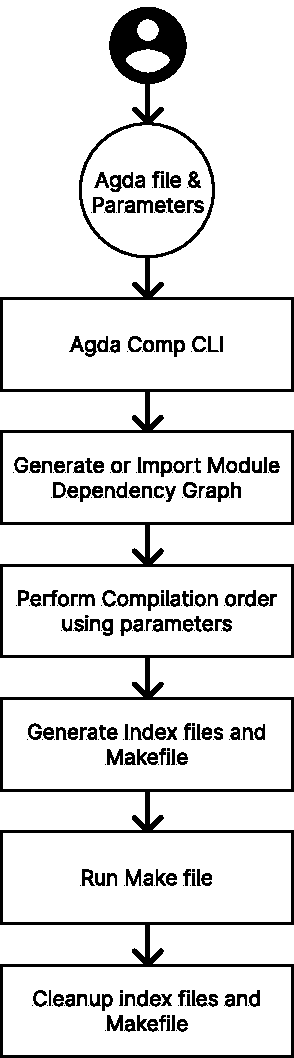
\includegraphics[scale=0.8]{Agda Comp.pdf}
    \caption{Agda Comp Diagram}
    \label{fig:Agda Comp Diagram}
\end{figure} 

\pagebreak
\subsection{Level Strategy} \label{sub:design level strategy}

The level strategy groups modules by their maximum distance from leaf nodes,
enabling parallel compilation within each level. Where leaf nodes at level
\(0\) and Level \(n\) depends on modules \(n - 1\) or below. This algorithm is
visualized in \cref{subfig: lvl strat}.
\begin{figure}[H]
  \begin{subfigure}[t]{0.45\textwidth}
    \centering
    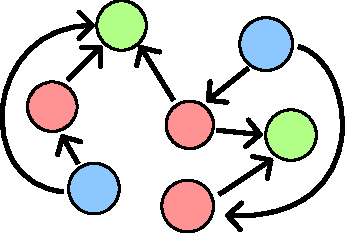
\includegraphics[scale=0.9]{lvl_graph.pdf}
    \caption{Example dependency graph}
    \label{fig:example lvl dep graph}
  \end{subfigure} \hfill
  \begin{subfigure}[t]{0.45\textwidth}
    \centering
    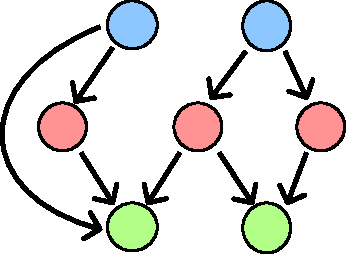
\includegraphics[scale=0.9]{lvl_sort.pdf}
    \caption{Example dependency graph sorted by levels where green means level
    0, red level 1 and blue level 2}
    \label{fig:example lvl sort}
  \end{subfigure}
  \caption{Level Strategy Example}
  \label{subfig: lvl strat}
\end{figure}

This strategy involves sorting modules into levels and compiling each level
sequentially, with concurrent compilation within levels which only depend on
previous levels. It guarantees that all modules in the dependency graph are
compiled, making the algorithm both safe and correct.

One advantage of this approach is it quickly generates the compilation order.
However, the strategy is limited. If a level contains only a few modules,
opportunities for parallel type-checking are low. Additionally, there are times
when two modules with distinct dependencies could be compiled in parallel,
leading to significant time savings with little overhead. However, this method
would first compile all shared dependencies before compiling these two modules
concurrently. This limitation becomes relevant during implementation
(\cref{sub:imp lvl strategy}), as the overhead associated with parallelization
can outweigh its benefits.


% \begin{itemize}
% \item What level ssortin is, connection to topo sort 
% \item Image of what the level means 
% \item How this is safe and correct from module dependency graph 
% \item How this finds parallel moduels
% \end{itemize}


\pagebreak
\subsection{Level Disjoint Strategy} \label{sub:design disjoint strategy}


The level disjoint strategy targets the weakness of the level sort strategy by
finding modules with many dependencies that can be compiled in parallel. It
identifies disjoint modules—those with distinct dependencies—and compiles them
concurrently. If no such modules are found, leaf nodes (modules with no
dependencies) are compiled first, and then it repeats. Once a module is
compiled, it no longer considered. This approach reduces the number of modules
to compile at each step and ensures all modules are eventually compiled. The
is illustrated in \cref{subfig:disj strat}.
\begin{figure}[H]
  \begin{subfigure}[t]{0.5\textwidth}
    \centering
    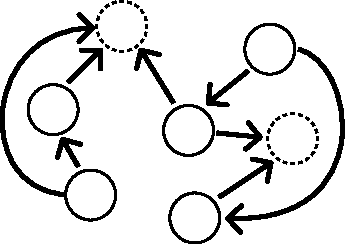
\includegraphics[scale=0.9]{disj_graph.pdf}
    \caption{Example dependency graph}
    \label{fig:example disj dep graph}
  \end{subfigure} \hfill
  \begin{subfigure}[t]{0.40\textwidth}
    \centering
    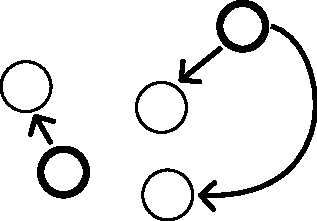
\includegraphics[scale=0.9]{disj_strat.pdf}
    \caption{Example dependency graph sorted where the leafs were removed,
    creating two modules that can be compiled in parallel. }
    \label{fig:example disj strat}
  \end{subfigure}
  \caption{Level Disjoint Example}
  \label{subfig:disj strat}
\end{figure}

This strategy is both safe and correct, as it avoids compiling conflicting
modules and guarantees that all modules in a project are compiled. It better
manages parallelization overhead by targeting larger modules, reducing repeated
loading of interface files during compilation. However, identifying disjoint
modules is challenging for projects with many modules. A brute-force approach
is impractical, so a greedy algorithm is used to approximate disjoint groups.
This algorithm sorts modules based on their dependencies and groups them into
buckets of disjoint modules for parallel compilation. This approach won't find
the optimal solution and is further explained in \cref{sub:imp disj strategy}/

Despite its benefits, its benefit depends on project structure. Libraries like
unimath \cite{agda-unimath}, which consist of many smaller independent modules,
benefit more than libraries like TypeTopology \cite{type-topology}, which have
larger connected modules. 

% \begin{itemize}
% \item What level disjoint does
% \item Image of what it attemps to do
% \item How this is safe and correct from module dependency graph 
% \item How this finds parallel moduels 
% \item the greedy algorithm to find disjoint modules
% \end{itemize}


\pagebreak

\section{Conclusion}

The diagram in \cref{fig:Agda Tree Class Diagram} shows how the structure of
the program. \cref{fig:Agda Create Tree Diagram} and \cref{fig:Agda Tree Query
Diagram} also shows how the dependency graphs will be created and how the user
will interact with CLI. This structure is important to ensure that the CLI can
handle all the requirements and gives the project a solid foundation to refer
back to. 

The functionality of Agda Comp is modelled in Figure \cref{fig:Agda Comp
Diagram}, this structure allows the user to select what compilation strategy to
use and how many cores the compilation can use. Agda Comp is lets the user to
easily apply the compilation strategies which are modelled in \cref{sub:design
level strategy} and in \cref{sub:design disjoint strategy}, then are
implemented in \cref{ch:implementation}.

% Communicating how you think about the composition of your system and how it
% works. You might detail the ways in which the overall system will be broken
% down into subsystems. Detail should then be provided on the design of each of
% these subsystems.
%
% \begin{itemize} \item A system that turns agda into s-expressions \item A
% system that reads s-expressions and turns it into a graph \item A system that
% queries that graph \item A way to store the graph for future use
% \end{itemize}

